% Options for packages loaded elsewhere
\PassOptionsToPackage{unicode}{hyperref}
\PassOptionsToPackage{hyphens}{url}
%
\documentclass[
]{article}
\usepackage{amsmath,amssymb}
\usepackage{lmodern}
\usepackage{iftex}
\ifPDFTeX
  \usepackage[T1]{fontenc}
  \usepackage[utf8]{inputenc}
  \usepackage{textcomp} % provide euro and other symbols
\else % if luatex or xetex
  \usepackage{unicode-math}
  \defaultfontfeatures{Scale=MatchLowercase}
  \defaultfontfeatures[\rmfamily]{Ligatures=TeX,Scale=1}
\fi
% Use upquote if available, for straight quotes in verbatim environments
\IfFileExists{upquote.sty}{\usepackage{upquote}}{}
\IfFileExists{microtype.sty}{% use microtype if available
  \usepackage[]{microtype}
  \UseMicrotypeSet[protrusion]{basicmath} % disable protrusion for tt fonts
}{}
\makeatletter
\@ifundefined{KOMAClassName}{% if non-KOMA class
  \IfFileExists{parskip.sty}{%
    \usepackage{parskip}
  }{% else
    \setlength{\parindent}{0pt}
    \setlength{\parskip}{6pt plus 2pt minus 1pt}}
}{% if KOMA class
  \KOMAoptions{parskip=half}}
\makeatother
\usepackage{xcolor}
\usepackage[margin=1in]{geometry}
\usepackage{color}
\usepackage{fancyvrb}
\newcommand{\VerbBar}{|}
\newcommand{\VERB}{\Verb[commandchars=\\\{\}]}
\DefineVerbatimEnvironment{Highlighting}{Verbatim}{commandchars=\\\{\}}
% Add ',fontsize=\small' for more characters per line
\usepackage{framed}
\definecolor{shadecolor}{RGB}{248,248,248}
\newenvironment{Shaded}{\begin{snugshade}}{\end{snugshade}}
\newcommand{\AlertTok}[1]{\textcolor[rgb]{0.94,0.16,0.16}{#1}}
\newcommand{\AnnotationTok}[1]{\textcolor[rgb]{0.56,0.35,0.01}{\textbf{\textit{#1}}}}
\newcommand{\AttributeTok}[1]{\textcolor[rgb]{0.77,0.63,0.00}{#1}}
\newcommand{\BaseNTok}[1]{\textcolor[rgb]{0.00,0.00,0.81}{#1}}
\newcommand{\BuiltInTok}[1]{#1}
\newcommand{\CharTok}[1]{\textcolor[rgb]{0.31,0.60,0.02}{#1}}
\newcommand{\CommentTok}[1]{\textcolor[rgb]{0.56,0.35,0.01}{\textit{#1}}}
\newcommand{\CommentVarTok}[1]{\textcolor[rgb]{0.56,0.35,0.01}{\textbf{\textit{#1}}}}
\newcommand{\ConstantTok}[1]{\textcolor[rgb]{0.00,0.00,0.00}{#1}}
\newcommand{\ControlFlowTok}[1]{\textcolor[rgb]{0.13,0.29,0.53}{\textbf{#1}}}
\newcommand{\DataTypeTok}[1]{\textcolor[rgb]{0.13,0.29,0.53}{#1}}
\newcommand{\DecValTok}[1]{\textcolor[rgb]{0.00,0.00,0.81}{#1}}
\newcommand{\DocumentationTok}[1]{\textcolor[rgb]{0.56,0.35,0.01}{\textbf{\textit{#1}}}}
\newcommand{\ErrorTok}[1]{\textcolor[rgb]{0.64,0.00,0.00}{\textbf{#1}}}
\newcommand{\ExtensionTok}[1]{#1}
\newcommand{\FloatTok}[1]{\textcolor[rgb]{0.00,0.00,0.81}{#1}}
\newcommand{\FunctionTok}[1]{\textcolor[rgb]{0.00,0.00,0.00}{#1}}
\newcommand{\ImportTok}[1]{#1}
\newcommand{\InformationTok}[1]{\textcolor[rgb]{0.56,0.35,0.01}{\textbf{\textit{#1}}}}
\newcommand{\KeywordTok}[1]{\textcolor[rgb]{0.13,0.29,0.53}{\textbf{#1}}}
\newcommand{\NormalTok}[1]{#1}
\newcommand{\OperatorTok}[1]{\textcolor[rgb]{0.81,0.36,0.00}{\textbf{#1}}}
\newcommand{\OtherTok}[1]{\textcolor[rgb]{0.56,0.35,0.01}{#1}}
\newcommand{\PreprocessorTok}[1]{\textcolor[rgb]{0.56,0.35,0.01}{\textit{#1}}}
\newcommand{\RegionMarkerTok}[1]{#1}
\newcommand{\SpecialCharTok}[1]{\textcolor[rgb]{0.00,0.00,0.00}{#1}}
\newcommand{\SpecialStringTok}[1]{\textcolor[rgb]{0.31,0.60,0.02}{#1}}
\newcommand{\StringTok}[1]{\textcolor[rgb]{0.31,0.60,0.02}{#1}}
\newcommand{\VariableTok}[1]{\textcolor[rgb]{0.00,0.00,0.00}{#1}}
\newcommand{\VerbatimStringTok}[1]{\textcolor[rgb]{0.31,0.60,0.02}{#1}}
\newcommand{\WarningTok}[1]{\textcolor[rgb]{0.56,0.35,0.01}{\textbf{\textit{#1}}}}
\usepackage{graphicx}
\makeatletter
\def\maxwidth{\ifdim\Gin@nat@width>\linewidth\linewidth\else\Gin@nat@width\fi}
\def\maxheight{\ifdim\Gin@nat@height>\textheight\textheight\else\Gin@nat@height\fi}
\makeatother
% Scale images if necessary, so that they will not overflow the page
% margins by default, and it is still possible to overwrite the defaults
% using explicit options in \includegraphics[width, height, ...]{}
\setkeys{Gin}{width=\maxwidth,height=\maxheight,keepaspectratio}
% Set default figure placement to htbp
\makeatletter
\def\fps@figure{htbp}
\makeatother
\setlength{\emergencystretch}{3em} % prevent overfull lines
\providecommand{\tightlist}{%
  \setlength{\itemsep}{0pt}\setlength{\parskip}{0pt}}
\setcounter{secnumdepth}{-\maxdimen} % remove section numbering
\ifLuaTeX
  \usepackage{selnolig}  % disable illegal ligatures
\fi
\IfFileExists{bookmark.sty}{\usepackage{bookmark}}{\usepackage{hyperref}}
\IfFileExists{xurl.sty}{\usepackage{xurl}}{} % add URL line breaks if available
\urlstyle{same} % disable monospaced font for URLs
\hypersetup{
  pdftitle={Math189 Final Project},
  pdfauthor={Daria Barbour-Brown},
  hidelinks,
  pdfcreator={LaTeX via pandoc}}

\title{Math189 Final Project}
\author{Daria Barbour-Brown}
\date{2023-05-25}

\begin{document}
\maketitle

\hypertarget{application-problems}{%
\section{Application Problems}\label{application-problems}}

\hypertarget{question-1}{%
\subsection{Question 1}\label{question-1}}

\emph{Consider the Carseats data in the ISLR2 package.}

\hypertarget{part-a}{%
\subsubsection{Part A}\label{part-a}}

\emph{Fit a linear regression model with Sales as the response and all
other variables as covariates. Report the coefficient estimates.}

\begin{Shaded}
\begin{Highlighting}[]
\CommentTok{\# Loading Carseat Data}
\FunctionTok{library}\NormalTok{(ISLR2)}
\FunctionTok{data}\NormalTok{(}\StringTok{"Carseats"}\NormalTok{)}
\end{Highlighting}
\end{Shaded}

\begin{Shaded}
\begin{Highlighting}[]
\CommentTok{\# Fit Linear Regression Model}
\NormalTok{lm.fit }\OtherTok{\textless{}{-}} \FunctionTok{lm}\NormalTok{(Sales }\SpecialCharTok{\textasciitilde{}}\NormalTok{ ., }\AttributeTok{data =}\NormalTok{ Carseats)}

\CommentTok{\# Report Coefficient Estimates}
\FunctionTok{summary}\NormalTok{(lm.fit)}
\end{Highlighting}
\end{Shaded}

\begin{verbatim}
## 
## Call:
## lm(formula = Sales ~ ., data = Carseats)
## 
## Residuals:
##     Min      1Q  Median      3Q     Max 
## -2.8692 -0.6908  0.0211  0.6636  3.4115 
## 
## Coefficients:
##                   Estimate Std. Error t value Pr(>|t|)    
## (Intercept)      5.6606231  0.6034487   9.380  < 2e-16 ***
## CompPrice        0.0928153  0.0041477  22.378  < 2e-16 ***
## Income           0.0158028  0.0018451   8.565 2.58e-16 ***
## Advertising      0.1230951  0.0111237  11.066  < 2e-16 ***
## Population       0.0002079  0.0003705   0.561    0.575    
## Price           -0.0953579  0.0026711 -35.700  < 2e-16 ***
## ShelveLocGood    4.8501827  0.1531100  31.678  < 2e-16 ***
## ShelveLocMedium  1.9567148  0.1261056  15.516  < 2e-16 ***
## Age             -0.0460452  0.0031817 -14.472  < 2e-16 ***
## Education       -0.0211018  0.0197205  -1.070    0.285    
## UrbanYes         0.1228864  0.1129761   1.088    0.277    
## USYes           -0.1840928  0.1498423  -1.229    0.220    
## ---
## Signif. codes:  0 '***' 0.001 '**' 0.01 '*' 0.05 '.' 0.1 ' ' 1
## 
## Residual standard error: 1.019 on 388 degrees of freedom
## Multiple R-squared:  0.8734, Adjusted R-squared:  0.8698 
## F-statistic: 243.4 on 11 and 388 DF,  p-value: < 2.2e-16
\end{verbatim}

\begin{Shaded}
\begin{Highlighting}[]
\FunctionTok{coefficients}\NormalTok{(lm.fit)}
\end{Highlighting}
\end{Shaded}

\begin{verbatim}
##     (Intercept)       CompPrice          Income     Advertising      Population 
##    5.6606230631    0.0928153421    0.0158028363    0.1230950886    0.0002078771 
##           Price   ShelveLocGood ShelveLocMedium             Age       Education 
##   -0.0953579188    4.8501827110    1.9567148062   -0.0460451630   -0.0211018389 
##        UrbanYes           USYes 
##    0.1228863965   -0.1840928246
\end{verbatim}

\hypertarget{part-b}{%
\subsubsection{Part B}\label{part-b}}

\emph{Determine whether the linear model is appropriate.}

\begin{Shaded}
\begin{Highlighting}[]
\CommentTok{\# Linear Model Assumption Testing}
\FunctionTok{par}\NormalTok{(}\AttributeTok{mfrow =} \FunctionTok{c}\NormalTok{(}\DecValTok{2}\NormalTok{, }\DecValTok{2}\NormalTok{))}
\FunctionTok{plot}\NormalTok{(lm.fit)}
\end{Highlighting}
\end{Shaded}

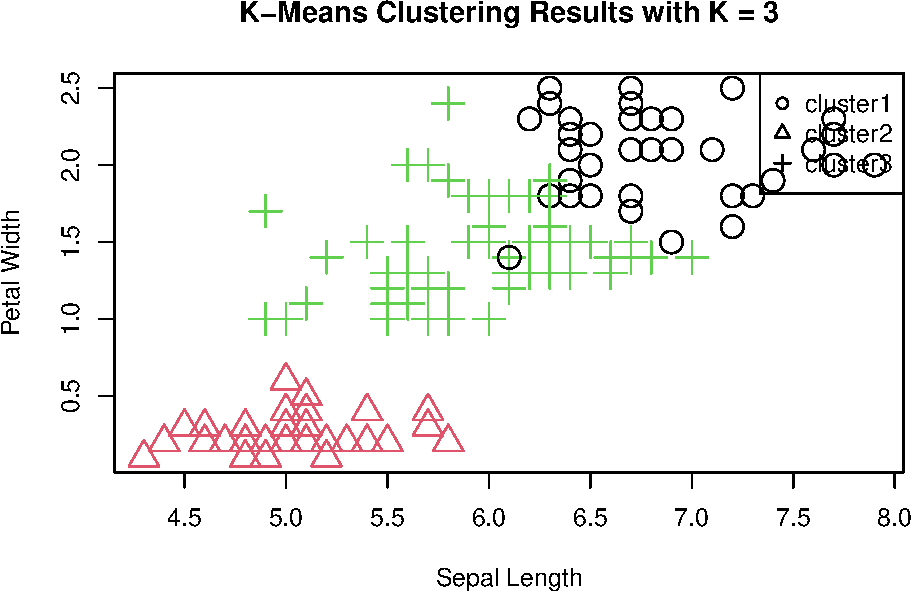
\includegraphics{189Final_NEW_files/figure-latex/unnamed-chunk-3-1.pdf}
We can determine the fitness of applying a linear model to our data by
observing the residual plots in order to test the assumptions for linear
regression. In our the above visualization, we plot our residuals
against the fitted values. In a residual plot for a linear model, you
typically look for certain patterns or characteristics that can help
assess the adequacy of the model. The spread of the residuals should
remain roughly constant across the range of predicted values. The
residuals should appear randomly scattered around the horizontal axis.
The residuals should be independent of each other, meaning that the
value of one residual should not provide any information about the value
of another residual. The residuals should not exhibit any systematic
curvature or nonlinear patterns. In our case, we see that none of these
conditions are violated, meaning that the data points do not seem to
show any systematic deviations from randomness.

Next we consider the Normal Q-Q plot. In a normal Q-Q plot, the
residuals are plotted against the quantiles of a theoretical normal
distribution. If the residuals are normally distributed, the points on
the plot should roughly follow a straight line. Departures from
normality can impact the accuracy of statistical tests and confidence
intervals associated with the model. In our case, our normality
assumption is met, given that our residuals follow the line denoting the
quantiles of a theoretical normal distribution. We conclude that fitting
a linear model is indeed appropriate.

\hypertarget{part-c}{%
\subsubsection{Part C}\label{part-c}}

\emph{Let beta-1 and beta-2 be the coefficients for CompPrice and
Income, respectively. Test the hypothesis that beta-1 = beta-2 = 0.
State your hypothesis, test statistic, and test statistic's distribution
clearly. Choose an alpha you feel is appropriate.}

\begin{Shaded}
\begin{Highlighting}[]
\DocumentationTok{\#\#\# ANOVA METHOD}

\FunctionTok{library}\NormalTok{(dplyr)}
\end{Highlighting}
\end{Shaded}

\begin{verbatim}
## 
## Attaching package: 'dplyr'
\end{verbatim}

\begin{verbatim}
## The following objects are masked from 'package:stats':
## 
##     filter, lag
\end{verbatim}

\begin{verbatim}
## The following objects are masked from 'package:base':
## 
##     intersect, setdiff, setequal, union
\end{verbatim}

\begin{Shaded}
\begin{Highlighting}[]
\NormalTok{data.subset }\OtherTok{=}\NormalTok{ Carseats[, }\SpecialCharTok{{-}}\FunctionTok{c}\NormalTok{(}\DecValTok{2}\NormalTok{,}\DecValTok{3}\NormalTok{)]}
\NormalTok{lmfit1 }\OtherTok{=} \FunctionTok{lm}\NormalTok{(Sales}\SpecialCharTok{\textasciitilde{}}\NormalTok{., }\AttributeTok{data=}\NormalTok{data.subset)}
\NormalTok{lmfit2 }\OtherTok{=} \FunctionTok{lm}\NormalTok{(Sales}\SpecialCharTok{\textasciitilde{}}\NormalTok{., }\AttributeTok{data=}\NormalTok{Carseats)}
\FunctionTok{anova}\NormalTok{(lmfit1,lmfit2)}
\end{Highlighting}
\end{Shaded}

\begin{verbatim}
## Analysis of Variance Table
## 
## Model 1: Sales ~ Advertising + Population + Price + ShelveLoc + Age + 
##     Education + Urban + US
## Model 2: Sales ~ CompPrice + Income + Advertising + Population + Price + 
##     ShelveLoc + Age + Education + Urban + US
##   Res.Df    RSS Df Sum of Sq      F    Pr(>F)    
## 1    390 977.31                                  
## 2    388 402.83  2    574.48 276.66 < 2.2e-16 ***
## ---
## Signif. codes:  0 '***' 0.001 '**' 0.01 '*' 0.05 '.' 0.1 ' ' 1
\end{verbatim}

Null hypothesis: There is no linear relationship between the predictor
variables and the response variable. In other words, the coefficients
for both CompPrice and Income are equal to zero.

Alternative hypothesis: There is a linear relationship between the
predictor variables and the response variable. At least one of the
coefficients for CompPrice or Income is not equal to zero.

The test statistics for each coefficient are represented by their
respective t-values. Meaning that our test statistic for CompPrice is
1.548, and 3.187 for Income.

The distribution of the test statistics is the t-distribution, which is
used in hypothesis testing for linear regression.

Since we are testing multiple hypotheses, we need to account for the
family-wise error rate. We do so by applying the Bonferroni-Holm
corrrection to our p-values.

Our resulting p-values are 0.1222 and 0.0023, for Carprice and Income,
respectively. Comparing our adjusted p-values to 95\% significance
level, \(\alpha\)=0.05, we can conclude that we should reject our null
hypothesis that both covariates are jointly equal to zero.

\hypertarget{question-2}{%
\subsection{Question 2}\label{question-2}}

\emph{Consider the Carseats data again.}

\hypertarget{part-a-1}{%
\subsubsection{Part A}\label{part-a-1}}

\emph{Split the data into a training set and a validation set. State the
proportions of your training/validation split.}

\begin{Shaded}
\begin{Highlighting}[]
\CommentTok{\# Define Variables}
\NormalTok{x }\OtherTok{\textless{}{-}} \FunctionTok{model.matrix}\NormalTok{(Sales }\SpecialCharTok{\textasciitilde{}}\NormalTok{ ., Carseats)[, }\SpecialCharTok{{-}}\DecValTok{1}\NormalTok{]}
\NormalTok{y }\OtherTok{\textless{}{-}}\NormalTok{ Carseats}\SpecialCharTok{$}\NormalTok{Sales}

\CommentTok{\# Train/Validation Split}
\FunctionTok{set.seed}\NormalTok{(}\DecValTok{1}\NormalTok{)}
\NormalTok{train }\OtherTok{\textless{}{-}} \FunctionTok{sample}\NormalTok{(}\DecValTok{1}\SpecialCharTok{:}\FunctionTok{nrow}\NormalTok{(x), }\FunctionTok{nrow}\NormalTok{(x) }\SpecialCharTok{*}\FloatTok{0.8}\NormalTok{)}
\NormalTok{test }\OtherTok{\textless{}{-}}\NormalTok{ (}\SpecialCharTok{{-}}\NormalTok{train)}
\NormalTok{y.test }\OtherTok{\textless{}{-}}\NormalTok{ y[test]}
\end{Highlighting}
\end{Shaded}

We will train our model on 80 percent of our data. The validation(test)
set will be comprised of the remaining 20 percent of unseen data.

\hypertarget{part-b-1}{%
\subsubsection{Part B}\label{part-b-1}}

\emph{Fit a ridge regression model on the training data, choosing the
lambda by cross-validation and reporting the final coefficients. Choose
an appropriate value for K when doing cross-validation.}

\begin{Shaded}
\begin{Highlighting}[]
\FunctionTok{library}\NormalTok{(glmnet)}
\end{Highlighting}
\end{Shaded}

\begin{verbatim}
## Loading required package: Matrix
\end{verbatim}

\begin{verbatim}
## Loaded glmnet 4.1-7
\end{verbatim}

\begin{Shaded}
\begin{Highlighting}[]
\NormalTok{rr.fit }\OtherTok{\textless{}{-}} \FunctionTok{cv.glmnet}\NormalTok{(x[train, ], y[train], }\AttributeTok{alpha =} \DecValTok{0}\NormalTok{, }\AttributeTok{nfolds =} \DecValTok{10}\NormalTok{) }
\end{Highlighting}
\end{Shaded}

\begin{Shaded}
\begin{Highlighting}[]
\CommentTok{\# Report best lambda}
\NormalTok{bestLambda }\OtherTok{\textless{}{-}}\NormalTok{ rr.fit}\SpecialCharTok{$}\NormalTok{lambda.min}
\NormalTok{bestLambda}
\end{Highlighting}
\end{Shaded}

\begin{verbatim}
## [1] 0.1395915
\end{verbatim}

\begin{Shaded}
\begin{Highlighting}[]
\CommentTok{\#Run ridge regression with best lambda, report coefficients}
\NormalTok{ridge.mod }\OtherTok{\textless{}{-}} \FunctionTok{glmnet}\NormalTok{(x, y, }\AttributeTok{alpha =} \DecValTok{0}\NormalTok{, }\AttributeTok{lambda =}\NormalTok{ bestLambda)}
\FunctionTok{coef}\NormalTok{(ridge.mod)}
\end{Highlighting}
\end{Shaded}

\begin{verbatim}
## 12 x 1 sparse Matrix of class "dgCMatrix"
##                            s0
## (Intercept)      6.3017064310
## CompPrice        0.0808046540
## Income           0.0146693896
## Advertising      0.1117261077
## Population       0.0001902178
## Price           -0.0861049868
## ShelveLocGood    4.4232806820
## ShelveLocMedium  1.6747315661
## Age             -0.0434522076
## Education       -0.0209803748
## UrbanYes         0.0972233371
## USYes           -0.0760578845
\end{verbatim}

\hypertarget{part-c-1}{%
\subsubsection{Part C}\label{part-c-1}}

\emph{Report the RMSE using the validation set on the model from 2b.}

\begin{Shaded}
\begin{Highlighting}[]
\CommentTok{\# Predict values using new X\textquotesingle{}s}
\NormalTok{ridge.pred }\OtherTok{\textless{}{-}} \FunctionTok{predict}\NormalTok{(ridge.mod, }\AttributeTok{s =}\NormalTok{ bestLambda, }\AttributeTok{newx =}\NormalTok{ x[test, ])}

\CommentTok{\# Calculating RMSE Root Mean Square Error}
\FunctionTok{sqrt}\NormalTok{(}\FunctionTok{mean}\NormalTok{((ridge.pred }\SpecialCharTok{{-}}\NormalTok{ y.test)}\SpecialCharTok{\^{}}\DecValTok{2}\NormalTok{))}
\end{Highlighting}
\end{Shaded}

\begin{verbatim}
## [1] 0.9883017
\end{verbatim}

\hypertarget{part-d}{%
\subsubsection{Part D}\label{part-d}}

\emph{Fit a random forest model on the training data, and report the
RMSE on the validation set.}

\begin{Shaded}
\begin{Highlighting}[]
\CommentTok{\#fit using training }
\FunctionTok{library}\NormalTok{(caret)}
\end{Highlighting}
\end{Shaded}

\begin{verbatim}
## Loading required package: ggplot2
\end{verbatim}

\begin{verbatim}
## Loading required package: lattice
\end{verbatim}

\begin{Shaded}
\begin{Highlighting}[]
\FunctionTok{library}\NormalTok{(randomForest)}
\end{Highlighting}
\end{Shaded}

\begin{verbatim}
## randomForest 4.7-1.1
\end{verbatim}

\begin{verbatim}
## Type rfNews() to see new features/changes/bug fixes.
\end{verbatim}

\begin{verbatim}
## 
## Attaching package: 'randomForest'
\end{verbatim}

\begin{verbatim}
## The following object is masked from 'package:ggplot2':
## 
##     margin
\end{verbatim}

\begin{verbatim}
## The following object is masked from 'package:dplyr':
## 
##     combine
\end{verbatim}

\begin{Shaded}
\begin{Highlighting}[]
\FunctionTok{set.seed}\NormalTok{(}\DecValTok{1}\NormalTok{)}

\NormalTok{rf.carseats }\OtherTok{\textless{}{-}} \FunctionTok{randomForest}\NormalTok{(Sales }\SpecialCharTok{\textasciitilde{}}\NormalTok{ ., }\AttributeTok{data =}\NormalTok{ Carseats, }\AttributeTok{subset =}\NormalTok{ train, }\AttributeTok{mtry =} \DecValTok{4}\NormalTok{, }\AttributeTok{importance =} \ConstantTok{TRUE}\NormalTok{)  }
\NormalTok{rf.predict }\OtherTok{\textless{}{-}} \FunctionTok{predict}\NormalTok{(rf.carseats, }\AttributeTok{newdata =}\NormalTok{ Carseats[test, ])}

\CommentTok{\#get RMSE using test}
\FunctionTok{sqrt}\NormalTok{(}\FunctionTok{mean}\NormalTok{((rf.predict }\SpecialCharTok{{-}}\NormalTok{ y.test)}\SpecialCharTok{\^{}}\DecValTok{2}\NormalTok{))}
\end{Highlighting}
\end{Shaded}

\begin{verbatim}
## [1] 1.78617
\end{verbatim}

\hypertarget{part-e}{%
\subsubsection{Part E}\label{part-e}}

\emph{For both of the models you fit in (b) and (d), give an example why
a marketing team would prefer one model over the other.}

Suppose a marketing team seeks a model that balances accurate
predictions with interpretability. Ridge regression meets their
requirements by providing interpretable coefficient estimates, allowing
them to assess the impact of predictors on customer satisfaction. This
aids in identifying influential variables and making informed decisions.
Additionally, ridge regression is a straightforward and transparent
linear model, simplifying communication with stakeholders. Moreover, in
our case, the ridge regression model performs better, exhibiting the
lowest root mean square error compared to our random forest model.
Hence, based on its simplicity and accuracy, we believe the marketing
team is likely to prefer the ridge regression model.

\hypertarget{question-3}{%
\subsection{Question 3}\label{question-3}}

\emph{In this question, you will simulate data to perform regression
between X and Y.}

\hypertarget{part-a-2}{%
\subsubsection{Part A}\label{part-a-2}}

\emph{Use the rt() function to generate a predictor X of length n=200.
Set df=15 for X}

\begin{Shaded}
\begin{Highlighting}[]
\FunctionTok{set.seed}\NormalTok{(}\DecValTok{1}\NormalTok{)}
\NormalTok{X }\OtherTok{\textless{}{-}} \FunctionTok{rt}\NormalTok{(}\AttributeTok{n=}\DecValTok{200}\NormalTok{, }\AttributeTok{df=}\DecValTok{15}\NormalTok{)}
\NormalTok{sorted\_idx }\OtherTok{=} \FunctionTok{order}\NormalTok{(X)}
\NormalTok{X }\OtherTok{=}\NormalTok{ X[sorted\_idx]}
\end{Highlighting}
\end{Shaded}

\hypertarget{part-b-2}{%
\subsubsection{Part B}\label{part-b-2}}

\emph{Use rt() to generate a noise vector epsilon. Set df=5.}

\begin{Shaded}
\begin{Highlighting}[]
\NormalTok{epsilon }\OtherTok{\textless{}{-}} \FunctionTok{rt}\NormalTok{(}\AttributeTok{n=}\DecValTok{200}\NormalTok{, }\AttributeTok{df=}\DecValTok{5}\NormalTok{)}
\end{Highlighting}
\end{Shaded}

\hypertarget{part-c-2}{%
\subsubsection{Part C}\label{part-c-2}}

*Generate a response vector Y of length n according to: Y=5+2sin(X)−
\frac{(7*\exp(2*cos(X)}{1+\exp(2*cos(X)} +\epsilon*

\begin{Shaded}
\begin{Highlighting}[]
\NormalTok{Y }\OtherTok{\textless{}{-}} \DecValTok{5}\SpecialCharTok{+}\DecValTok{2}\SpecialCharTok{*}\FunctionTok{sin}\NormalTok{(X)}\SpecialCharTok{{-}}\NormalTok{(}\DecValTok{7}\SpecialCharTok{*}\NormalTok{(}\FunctionTok{exp}\NormalTok{(}\DecValTok{2}\SpecialCharTok{*}\FunctionTok{cos}\NormalTok{(X))}\SpecialCharTok{/}\NormalTok{(}\DecValTok{1}\SpecialCharTok{+}\FunctionTok{exp}\NormalTok{(}\DecValTok{2}\SpecialCharTok{*}\FunctionTok{cos}\NormalTok{(X))))) }\SpecialCharTok{+}\NormalTok{ epsilon}
\end{Highlighting}
\end{Shaded}

\hypertarget{part-d-1}{%
\subsubsection{Part D}\label{part-d-1}}

\emph{Fit polynomial regression for Y on X with the order of X ranging
from 1 to 5.
(i.e.Y=β0+β1X+ϵ,Y=β0+β1X+β2X2+ϵ,\ldots,Y=β0+β1X+β2X2β3X3+β4X4+β5X5+ϵ)
and plot each of the five model fits, in different colors and with a
legend, on top of your simulated data.}

\begin{Shaded}
\begin{Highlighting}[]
\FunctionTok{plot}\NormalTok{(X, Y)}
\NormalTok{colors }\OtherTok{\textless{}{-}} \FunctionTok{sample}\NormalTok{(}\FunctionTok{colors}\NormalTok{(), }\DecValTok{5}\NormalTok{)}
\NormalTok{legend\_labels }\OtherTok{\textless{}{-}} \FunctionTok{c}\NormalTok{()}

\ControlFlowTok{for}\NormalTok{ (p }\ControlFlowTok{in} \DecValTok{1}\SpecialCharTok{:}\DecValTok{5}\NormalTok{) \{}
\NormalTok{  fit }\OtherTok{\textless{}{-}} \FunctionTok{lm}\NormalTok{(Y }\SpecialCharTok{\textasciitilde{}} \FunctionTok{poly}\NormalTok{(X, p))}
\NormalTok{  val }\OtherTok{\textless{}{-}} \FunctionTok{predict}\NormalTok{(fit, }\FunctionTok{data.frame}\NormalTok{(}\AttributeTok{X =}\NormalTok{ X))}
  \FunctionTok{lines}\NormalTok{(X, val, }\AttributeTok{col =}\NormalTok{ colors[p], }\AttributeTok{lwd =} \DecValTok{2}\NormalTok{)}
\NormalTok{  legend\_labels }\OtherTok{\textless{}{-}} \FunctionTok{c}\NormalTok{(legend\_labels, }\FunctionTok{paste0}\NormalTok{(}\StringTok{"Degree "}\NormalTok{, p))}
\NormalTok{\}}

\FunctionTok{legend}\NormalTok{(}\StringTok{"topright"}\NormalTok{, }\AttributeTok{legend =}\NormalTok{ legend\_labels, }\AttributeTok{col =}\NormalTok{ colors, }\AttributeTok{lwd =} \DecValTok{2}\NormalTok{)}
\end{Highlighting}
\end{Shaded}

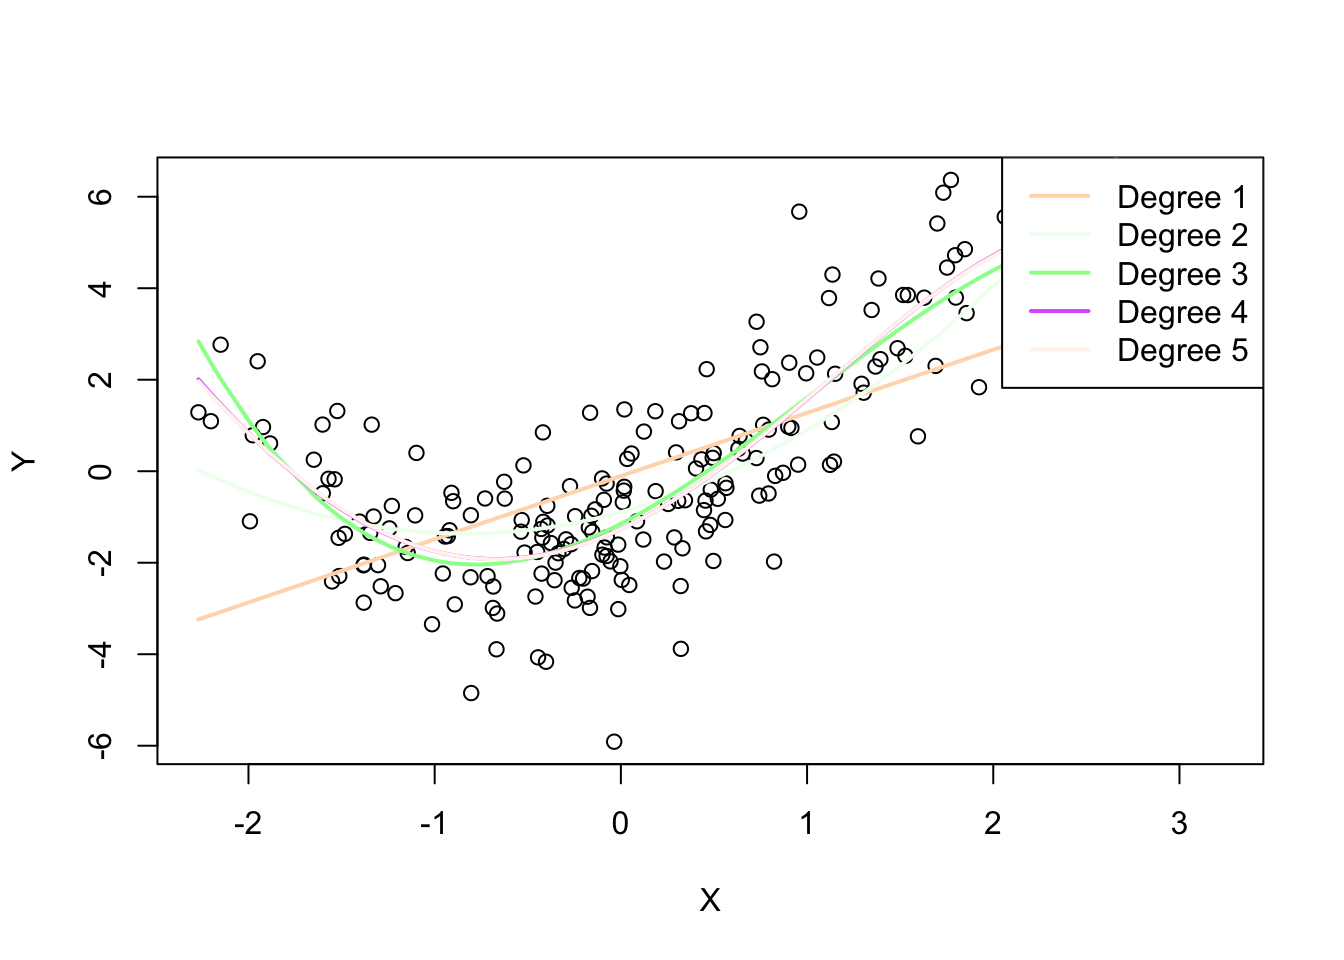
\includegraphics{189Final_NEW_files/figure-latex/unnamed-chunk-13-1.pdf}

\hypertarget{part-e-1}{%
\subsubsection{Part E}\label{part-e-1}}

\emph{Which one of these models do you prefer? Justify your answer.} We
utilize 10-fold cross validation to determine the most suitable
polynomial for our data. Through this process, we identify that the
polynomial with degree 5 yields the smallest validation/prediction
error. The corresponding visualization of this final polynomial can be
observed in the plot below.

\begin{Shaded}
\begin{Highlighting}[]
\FunctionTok{library}\NormalTok{(boot)}
\end{Highlighting}
\end{Shaded}

\begin{verbatim}
## 
## Attaching package: 'boot'
\end{verbatim}

\begin{verbatim}
## The following object is masked from 'package:lattice':
## 
##     melanoma
\end{verbatim}

\begin{Shaded}
\begin{Highlighting}[]
\FunctionTok{set.seed}\NormalTok{ (}\DecValTok{1}\NormalTok{)}
\NormalTok{df }\OtherTok{=} \FunctionTok{cbind.data.frame}\NormalTok{(X,Y)}
\NormalTok{predErr }\OtherTok{\textless{}{-}} \FunctionTok{rep}\NormalTok{ (}\DecValTok{0}\NormalTok{, }\DecValTok{5}\NormalTok{)}
\ControlFlowTok{for}\NormalTok{ (i }\ControlFlowTok{in} \DecValTok{1}\SpecialCharTok{:}\DecValTok{5}\NormalTok{) \{}
\NormalTok{  glm.fit }\OtherTok{\textless{}{-}} \FunctionTok{glm}\NormalTok{(Y}\SpecialCharTok{\textasciitilde{}}\FunctionTok{poly}\NormalTok{(X,i), }\AttributeTok{data =}\NormalTok{ df)}
\NormalTok{  predErr[i] }\OtherTok{\textless{}{-}} \FunctionTok{cv.glm}\NormalTok{ (df , glm.fit , }\AttributeTok{K =} \DecValTok{10}\NormalTok{)}\SpecialCharTok{$}\NormalTok{delta[}\DecValTok{1}\NormalTok{]}
\NormalTok{\}}
\NormalTok{predErr}
\end{Highlighting}
\end{Shaded}

\begin{verbatim}
## [1] 3.416248 2.375047 1.724267 1.688903 1.681169
\end{verbatim}

\begin{Shaded}
\begin{Highlighting}[]
\FunctionTok{min}\NormalTok{(predErr)}
\end{Highlighting}
\end{Shaded}

\begin{verbatim}
## [1] 1.681169
\end{verbatim}

\hypertarget{part-f}{%
\subsubsection{Part F}\label{part-f}}

\emph{For the model Y=β0+β1X+β2X2+ϵ, compute a 90\% confidence interval
at X=1 using least squares theory. Provide an interpretation for this
interval.}

\begin{Shaded}
\begin{Highlighting}[]
\NormalTok{fit }\OtherTok{=} \FunctionTok{lm}\NormalTok{(Y }\SpecialCharTok{\textasciitilde{}} \FunctionTok{poly}\NormalTok{(X,}\DecValTok{2}\NormalTok{))}
\NormalTok{ci }\OtherTok{=} \FunctionTok{predict}\NormalTok{(fit, }\FunctionTok{data.frame}\NormalTok{(}\AttributeTok{X=}\DecValTok{1}\NormalTok{), }\AttributeTok{level =} \FloatTok{0.90}\NormalTok{, }\AttributeTok{interval =} \StringTok{"confidence"}\NormalTok{)}
\NormalTok{ci}
\end{Highlighting}
\end{Shaded}

\begin{verbatim}
##         fit       lwr      upr
## 1 0.9029684 0.6640983 1.141839
\end{verbatim}

90\% CI: {[}0.6640983, 1.141839{]}

Our Confidence Interval indicates that in around 90\% of cases, the true
value of the response variable (when X=1) would lie within this interval
if we were to replicate the data collection and modeling process
multiple times.

\hypertarget{part-g}{%
\subsubsection{Part G}\label{part-g}}

\emph{For the model Y=β0+β1X+β2X2+ϵ, compute a 90\% confidence interval
at X=1 using a bootstrap. Provide an interpretation for this interval.}

\begin{Shaded}
\begin{Highlighting}[]
\NormalTok{df}\OtherTok{=}\FunctionTok{data.frame}\NormalTok{(}\AttributeTok{Y=}\NormalTok{Y,}\AttributeTok{X=}\NormalTok{X)}

\CommentTok{\# Set the number of bootstrap samples}
\NormalTok{B }\OtherTok{\textless{}{-}} \DecValTok{200}

\CommentTok{\# Vector to store bootstrap estimates}
\NormalTok{bootstrap\_estimates }\OtherTok{\textless{}{-}} \FunctionTok{numeric}\NormalTok{(B)  }

\CommentTok{\#Bootstrp Procedure}

\ControlFlowTok{for}\NormalTok{ (b }\ControlFlowTok{in} \DecValTok{1}\SpecialCharTok{:}\NormalTok{B) \{}
  \CommentTok{\# Sample with replacement from the original dataset}
\NormalTok{  bootstrap\_data }\OtherTok{\textless{}{-}}\NormalTok{ df[}\FunctionTok{sample}\NormalTok{(}\FunctionTok{nrow}\NormalTok{(df), }\AttributeTok{replace =} \ConstantTok{TRUE}\NormalTok{), ]}
  
  \CommentTok{\# Fit the model on the bootstrap sample}
\NormalTok{  fit }\OtherTok{\textless{}{-}} \FunctionTok{lm}\NormalTok{(Y }\SpecialCharTok{\textasciitilde{}} \FunctionTok{poly}\NormalTok{(X, }\DecValTok{2}\NormalTok{), }\AttributeTok{data =}\NormalTok{ bootstrap\_data)}
  
  \CommentTok{\# Predict the response at X = 1}
\NormalTok{  bootstrap\_estimates[b] }\OtherTok{\textless{}{-}} \FunctionTok{predict}\NormalTok{(fit, }\AttributeTok{newdata =} \FunctionTok{data.frame}\NormalTok{(}\AttributeTok{X =} \DecValTok{1}\NormalTok{))}
\NormalTok{\}}

\NormalTok{confidence\_interval }\OtherTok{\textless{}{-}} \FunctionTok{quantile}\NormalTok{(bootstrap\_estimates, }\FunctionTok{c}\NormalTok{(}\FloatTok{0.05}\NormalTok{, }\FloatTok{0.95}\NormalTok{))}
\NormalTok{confidence\_interval}
\end{Highlighting}
\end{Shaded}

\begin{verbatim}
##        5%       95% 
## 0.6498244 1.1400490
\end{verbatim}

The confidence interval provides valuable insights into the likely range
of the model's prediction at X = 1. It takes into consideration the
data's variability and the estimation process through bootstrapping.
Upon repeating the bootstrapping procedure multiple times, approximately
90\% of the calculated confidence intervals would encompass the true
value of the model's prediction at X = 1. The lower bound of the
interval represents the estimated minimum value, while the upper bound
represents the estimated maximum value. In simpler terms, the confidence
interval offers a reasonable range within which we can anticipate the
model's prediction at X = 1 to fall.

\hypertarget{question-4}{%
\subsection{Question 4}\label{question-4}}

\emph{Consider the College data set in the ISLR2 package.}

\hypertarget{part-a-3}{%
\subsubsection{Part A}\label{part-a-3}}

\emph{Split the data set into a training and validation set.}

\begin{Shaded}
\begin{Highlighting}[]
\FunctionTok{data}\NormalTok{(College)}
\end{Highlighting}
\end{Shaded}

\begin{Shaded}
\begin{Highlighting}[]
\FunctionTok{set.seed}\NormalTok{(}\DecValTok{4}\NormalTok{)}
\NormalTok{train }\OtherTok{=} \FunctionTok{sample}\NormalTok{(}\FunctionTok{nrow}\NormalTok{(College), }\FunctionTok{nrow}\NormalTok{(College)}\SpecialCharTok{*}\NormalTok{.}\DecValTok{8}\NormalTok{)}
\NormalTok{train\_set }\OtherTok{\textless{}{-}}\NormalTok{ College[train, ]}
\NormalTok{valid\_set }\OtherTok{\textless{}{-}}\NormalTok{ College[}\SpecialCharTok{{-}}\NormalTok{train, ]}
\end{Highlighting}
\end{Shaded}

\hypertarget{part-b-3}{%
\subsubsection{Part B}\label{part-b-3}}

\emph{Perform logistic regression on the training data to predict the
variable Private using all other variables. Provide an interpretation of
the coefficient for Top10Perc.}

\begin{Shaded}
\begin{Highlighting}[]
\NormalTok{logRegMulti }\OtherTok{\textless{}{-}} \FunctionTok{glm}\NormalTok{(Private }\SpecialCharTok{\textasciitilde{}}\NormalTok{ ., }\AttributeTok{data=}\NormalTok{College, }\AttributeTok{family=}\StringTok{"binomial"}\NormalTok{)}
\FunctionTok{summary}\NormalTok{(logRegMulti)}
\end{Highlighting}
\end{Shaded}

\begin{verbatim}
## 
## Call:
## glm(formula = Private ~ ., family = "binomial", data = College)
## 
## Deviance Residuals: 
##     Min       1Q   Median       3Q      Max  
## -3.7673  -0.0318   0.0502   0.1717   4.2070  
## 
## Coefficients:
##               Estimate Std. Error z value Pr(>|z|)    
## (Intercept) -2.574e-02  1.860e+00  -0.014  0.98896    
## Apps        -5.138e-04  2.284e-04  -2.249  0.02452 *  
## Accept       9.328e-05  4.382e-04   0.213  0.83144    
## Enroll       1.331e-03  8.487e-04   1.568  0.11687    
## Top10perc    8.451e-03  2.841e-02   0.297  0.76614    
## Top25perc    7.305e-03  1.895e-02   0.385  0.69993    
## F.Undergrad -4.168e-04  1.472e-04  -2.832  0.00462 ** 
## P.Undergrad  1.836e-05  1.348e-04   0.136  0.89164    
## Outstate     6.822e-04  1.099e-04   6.207  5.4e-10 ***
## Room.Board   1.901e-04  2.575e-04   0.738  0.46053    
## Books        2.059e-03  1.318e-03   1.562  0.11837    
## Personal    -3.283e-04  2.700e-04  -1.216  0.22395    
## PhD         -6.027e-02  2.665e-02  -2.262  0.02371 *  
## Terminal    -3.590e-02  2.580e-02  -1.392  0.16402    
## S.F.Ratio   -8.461e-02  6.076e-02  -1.393  0.16372    
## perc.alumni  4.782e-02  2.097e-02   2.280  0.02260 *  
## Expend       2.077e-04  1.207e-04   1.721  0.08529 .  
## Grad.Rate    1.634e-02  1.171e-02   1.395  0.16294    
## ---
## Signif. codes:  0 '***' 0.001 '**' 0.01 '*' 0.05 '.' 0.1 ' ' 1
## 
## (Dispersion parameter for binomial family taken to be 1)
## 
##     Null deviance: 910.75  on 776  degrees of freedom
## Residual deviance: 239.50  on 759  degrees of freedom
## AIC: 275.5
## 
## Number of Fisher Scoring iterations: 8
\end{verbatim}

\begin{Shaded}
\begin{Highlighting}[]
\FunctionTok{exp}\NormalTok{(}\FunctionTok{coefficients}\NormalTok{(logRegMulti))}
\end{Highlighting}
\end{Shaded}

\begin{verbatim}
## (Intercept)        Apps      Accept      Enroll   Top10perc   Top25perc 
##   0.9745854   0.9994864   1.0000933   1.0013317   1.0084863   1.0073315 
## F.Undergrad P.Undergrad    Outstate  Room.Board       Books    Personal 
##   0.9995833   1.0000184   1.0006824   1.0001901   1.0020609   0.9996717 
##         PhD    Terminal   S.F.Ratio perc.alumni      Expend   Grad.Rate 
##   0.9415102   0.9647323   0.9188665   1.0489822   1.0002077   1.0164721
\end{verbatim}

\(\beta_4\) = 8.451e-03 corresponding to Top10perc

The coefficient for the variable Top10perc suggests that a one-unit
increase in Top10perc is expected to result in a logarithmic odds
increase of around 0.008451 for the outcome variable. However, it is
crucial to highlight that this estimate does not achieve statistical
significance. This lack of significance implies that the observed
relationship between Top10perc and the outcome variable may not hold any
meaningful or distinguishable pattern from random variation.

\hypertarget{part-c-3}{%
\subsubsection{Part C}\label{part-c-3}}

\emph{What is the test error for the logistic regression (justify your
selection of your threshold)?}

\begin{Shaded}
\begin{Highlighting}[]
\CommentTok{\# Set the number of folds for cross{-}validation}
\NormalTok{num\_folds }\OtherTok{\textless{}{-}} \DecValTok{10}

\NormalTok{accuracy }\OtherTok{\textless{}{-}} \FunctionTok{numeric}\NormalTok{(num\_folds)}
\FunctionTok{set.seed}\NormalTok{(}\DecValTok{123}\NormalTok{)  }\CommentTok{\# For reproducibility}
\NormalTok{fold\_indices }\OtherTok{\textless{}{-}} \FunctionTok{sample}\NormalTok{(}\FunctionTok{rep}\NormalTok{(}\DecValTok{1}\SpecialCharTok{:}\NormalTok{num\_folds, }\AttributeTok{length.out =} \FunctionTok{nrow}\NormalTok{(College)))}

\CommentTok{\# Perform cross{-}validation}
\ControlFlowTok{for}\NormalTok{ (i }\ControlFlowTok{in} \DecValTok{1}\SpecialCharTok{:}\NormalTok{num\_folds) \{}
  \CommentTok{\# Split the data into training and test sets based on the fold indices}
\NormalTok{  train\_data }\OtherTok{\textless{}{-}}\NormalTok{ College[fold\_indices }\SpecialCharTok{!=}\NormalTok{ i, ]}
\NormalTok{  test\_data }\OtherTok{\textless{}{-}}\NormalTok{ College[fold\_indices }\SpecialCharTok{==}\NormalTok{ i, ]}
  
  \CommentTok{\# Fit logistic regression model on training data}
\NormalTok{  logreg\_model }\OtherTok{\textless{}{-}} \FunctionTok{glm}\NormalTok{(Private }\SpecialCharTok{\textasciitilde{}}\NormalTok{ ., }\AttributeTok{data =}\NormalTok{ train\_data, }\AttributeTok{family =} \StringTok{"binomial"}\NormalTok{)}
  
  \CommentTok{\# Predict on test data}
\NormalTok{  test\_preds }\OtherTok{\textless{}{-}} \FunctionTok{predict}\NormalTok{(logreg\_model, }\AttributeTok{newdata =}\NormalTok{ test\_data, }\AttributeTok{type =} \StringTok{"response"}\NormalTok{)}
\NormalTok{  test\_class\_preds }\OtherTok{\textless{}{-}} \FunctionTok{ifelse}\NormalTok{(test\_preds }\SpecialCharTok{\textgreater{}} \FloatTok{0.65}\NormalTok{, }\StringTok{"Yes"}\NormalTok{, }\StringTok{"No"}\NormalTok{)}
  
\NormalTok{  accuracy[i] }\OtherTok{\textless{}{-}} \FunctionTok{mean}\NormalTok{(test\_class\_preds }\SpecialCharTok{==}\NormalTok{ test\_data}\SpecialCharTok{$}\NormalTok{Private)}
\NormalTok{\}}
\end{Highlighting}
\end{Shaded}

\begin{verbatim}
## Warning: glm.fit: fitted probabilities numerically 0 or 1 occurred
\end{verbatim}

\begin{Shaded}
\begin{Highlighting}[]
\CommentTok{\#average test error}
\NormalTok{test\_error }\OtherTok{\textless{}{-}} \DecValTok{1} \SpecialCharTok{{-}} \FunctionTok{mean}\NormalTok{(accuracy)}
\FunctionTok{print}\NormalTok{(test\_error)}
\end{Highlighting}
\end{Shaded}

\begin{verbatim}
## [1] 0.06182151
\end{verbatim}

\begin{Shaded}
\begin{Highlighting}[]
\FunctionTok{library}\NormalTok{(pROC) }
\end{Highlighting}
\end{Shaded}

\begin{verbatim}
## Type 'citation("pROC")' for a citation.
\end{verbatim}

\begin{verbatim}
## 
## Attaching package: 'pROC'
\end{verbatim}

\begin{verbatim}
## The following objects are masked from 'package:stats':
## 
##     cov, smooth, var
\end{verbatim}

\begin{Shaded}
\begin{Highlighting}[]
\CommentTok{\# Fit logistic regression model on the entire dataset}
\NormalTok{logreg\_model }\OtherTok{\textless{}{-}} \FunctionTok{glm}\NormalTok{(Private }\SpecialCharTok{\textasciitilde{}}\NormalTok{ ., }\AttributeTok{data =}\NormalTok{ College, }\AttributeTok{family =} \StringTok{"binomial"}\NormalTok{)}
\NormalTok{pred\_probs }\OtherTok{\textless{}{-}} \FunctionTok{predict}\NormalTok{(logreg\_model, }\AttributeTok{type =} \StringTok{"response"}\NormalTok{)}

\CommentTok{\# Create a ROC object}
\NormalTok{roc.info }\OtherTok{\textless{}{-}} \FunctionTok{roc}\NormalTok{(College}\SpecialCharTok{$}\NormalTok{Private, pred\_probs, }\AttributeTok{legacy.axes =} \ConstantTok{TRUE}\NormalTok{)}
\end{Highlighting}
\end{Shaded}

\begin{verbatim}
## Setting levels: control = No, case = Yes
\end{verbatim}

\begin{verbatim}
## Setting direction: controls < cases
\end{verbatim}

\begin{Shaded}
\begin{Highlighting}[]
\NormalTok{roc.df }\OtherTok{\textless{}{-}} \FunctionTok{data.frame}\NormalTok{(}\AttributeTok{tpp =}\NormalTok{ roc.info}\SpecialCharTok{$}\NormalTok{sensitivities}\SpecialCharTok{*}\DecValTok{100}\NormalTok{, }\AttributeTok{fpp =}\NormalTok{ (}\DecValTok{1} \SpecialCharTok{{-}}\NormalTok{ roc.info}\SpecialCharTok{$}\NormalTok{specificities)}\SpecialCharTok{*}\DecValTok{100}\NormalTok{, }\AttributeTok{thresholds =}\NormalTok{ roc.info}\SpecialCharTok{$}\NormalTok{thresholds)}

\CommentTok{\# Get the coordinates of the point with the highest AUC}
\NormalTok{best\_coords }\OtherTok{\textless{}{-}} \FunctionTok{coords}\NormalTok{(roc.info, }\StringTok{"best"}\NormalTok{)}

\CommentTok{\# Extract the best threshold and corresponding AUC}
\NormalTok{best\_threshold }\OtherTok{\textless{}{-}}\NormalTok{ best\_coords}\SpecialCharTok{$}\NormalTok{threshold}
\NormalTok{best\_threshold}
\end{Highlighting}
\end{Shaded}

\begin{verbatim}
## [1] 0.6538537
\end{verbatim}

\begin{Shaded}
\begin{Highlighting}[]
\FunctionTok{plot.roc}\NormalTok{(College}\SpecialCharTok{$}\NormalTok{Private, }\FunctionTok{predict}\NormalTok{(logreg\_model, }\AttributeTok{type =} \StringTok{"response"}\NormalTok{), }\AttributeTok{legacy.axes =} \ConstantTok{TRUE}\NormalTok{, }\AttributeTok{percent =} \ConstantTok{TRUE}\NormalTok{, }\AttributeTok{xlab =} \StringTok{"False Pos Percentage"}\NormalTok{, }\AttributeTok{ylab =} \StringTok{"True Pos Percentage"}\NormalTok{)}
\end{Highlighting}
\end{Shaded}

\begin{verbatim}
## Setting levels: control = No, case = Yes
## Setting direction: controls < cases
\end{verbatim}

\includegraphics{189Final_NEW_files/figure-latex/unnamed-chunk-20-1.pdf}

\begin{Shaded}
\begin{Highlighting}[]
\DocumentationTok{\#\#\#\#\#\#\#\#\#\#\#\#\#\#\#\#\#\#\#\#\#\#}
\end{Highlighting}
\end{Shaded}

We ended up choosing \textbf{.65} as our threshold by selecting the
threshold corresponding to the best sum of sensitivity + specificity
respectively.

\hypertarget{part-d-2}{%
\subsubsection{Part D}\label{part-d-2}}

\emph{Fit an LDA to the same model, and report the test error.}

\begin{Shaded}
\begin{Highlighting}[]
\FunctionTok{library}\NormalTok{(MASS)}
\end{Highlighting}
\end{Shaded}

\begin{verbatim}
## 
## Attaching package: 'MASS'
\end{verbatim}

\begin{verbatim}
## The following object is masked from 'package:dplyr':
## 
##     select
\end{verbatim}

\begin{verbatim}
## The following object is masked from 'package:ISLR2':
## 
##     Boston
\end{verbatim}

\begin{Shaded}
\begin{Highlighting}[]
\NormalTok{num\_folds }\OtherTok{\textless{}{-}} \DecValTok{10}

\NormalTok{accuracy }\OtherTok{\textless{}{-}} \FunctionTok{numeric}\NormalTok{(num\_folds)}

\FunctionTok{set.seed}\NormalTok{(}\DecValTok{123}\NormalTok{) }
\NormalTok{fold\_indices }\OtherTok{\textless{}{-}} \FunctionTok{sample}\NormalTok{(}\FunctionTok{rep}\NormalTok{(}\DecValTok{1}\SpecialCharTok{:}\NormalTok{num\_folds, }\AttributeTok{length.out =} \FunctionTok{nrow}\NormalTok{(College)))}

\CommentTok{\#cross{-}validation}
\ControlFlowTok{for}\NormalTok{ (i }\ControlFlowTok{in} \DecValTok{1}\SpecialCharTok{:}\NormalTok{num\_folds) \{}
\NormalTok{  train\_data }\OtherTok{\textless{}{-}}\NormalTok{ College[fold\_indices }\SpecialCharTok{!=}\NormalTok{ i, ]}
\NormalTok{  test\_data }\OtherTok{\textless{}{-}}\NormalTok{ College[fold\_indices }\SpecialCharTok{==}\NormalTok{ i, ]}
  
  \CommentTok{\# Fit LDA model on training data}
\NormalTok{  lda\_model }\OtherTok{\textless{}{-}} \FunctionTok{lda}\NormalTok{(Private }\SpecialCharTok{\textasciitilde{}}\NormalTok{ ., }\AttributeTok{data =}\NormalTok{ train\_data)}
  
  \CommentTok{\# Predict on test data}
\NormalTok{  test\_preds }\OtherTok{\textless{}{-}} \FunctionTok{predict}\NormalTok{(lda\_model, }\AttributeTok{newdata =}\NormalTok{ test\_data)}
\NormalTok{  test\_class\_preds }\OtherTok{\textless{}{-}}\NormalTok{ test\_preds}\SpecialCharTok{$}\NormalTok{class}
  
\NormalTok{  accuracy[i] }\OtherTok{\textless{}{-}} \FunctionTok{mean}\NormalTok{(test\_class\_preds }\SpecialCharTok{==}\NormalTok{ test\_data}\SpecialCharTok{$}\NormalTok{Private)}
\NormalTok{\}}

\NormalTok{test\_error }\OtherTok{\textless{}{-}} \DecValTok{1} \SpecialCharTok{{-}} \FunctionTok{mean}\NormalTok{(accuracy)}
\FunctionTok{print}\NormalTok{(test\_error)}
\end{Highlighting}
\end{Shaded}

\begin{verbatim}
## [1] 0.06438561
\end{verbatim}

\hypertarget{part-e-2}{%
\subsubsection{Part E}\label{part-e-2}}

\emph{Fit an QDA to the same model, and report the test error.}

\begin{Shaded}
\begin{Highlighting}[]
\FunctionTok{library}\NormalTok{(MASS)}
\NormalTok{num\_folds }\OtherTok{\textless{}{-}} \DecValTok{10}
\NormalTok{accuracy }\OtherTok{\textless{}{-}} \FunctionTok{numeric}\NormalTok{(num\_folds)}

\FunctionTok{set.seed}\NormalTok{(}\DecValTok{123}\NormalTok{) }
\NormalTok{fold\_indices }\OtherTok{\textless{}{-}} \FunctionTok{sample}\NormalTok{(}\FunctionTok{rep}\NormalTok{(}\DecValTok{1}\SpecialCharTok{:}\NormalTok{num\_folds, }\AttributeTok{length.out =} \FunctionTok{nrow}\NormalTok{(College)))}

\ControlFlowTok{for}\NormalTok{ (i }\ControlFlowTok{in} \DecValTok{1}\SpecialCharTok{:}\NormalTok{num\_folds) \{}
\NormalTok{  train\_data }\OtherTok{\textless{}{-}}\NormalTok{ College[fold\_indices }\SpecialCharTok{!=}\NormalTok{ i, ]}
\NormalTok{  test\_data }\OtherTok{\textless{}{-}}\NormalTok{ College[fold\_indices }\SpecialCharTok{==}\NormalTok{ i, ]}
  
  \CommentTok{\# Fit QDA model on training data}
\NormalTok{  qda\_model }\OtherTok{\textless{}{-}} \FunctionTok{qda}\NormalTok{(Private }\SpecialCharTok{\textasciitilde{}}\NormalTok{ ., }\AttributeTok{data =}\NormalTok{ train\_data)}
  
  \CommentTok{\# Predict on test data}
\NormalTok{  test\_preds }\OtherTok{\textless{}{-}} \FunctionTok{predict}\NormalTok{(qda\_model, }\AttributeTok{newdata =}\NormalTok{ test\_data)}
\NormalTok{  test\_class\_preds }\OtherTok{\textless{}{-}}\NormalTok{ test\_preds}\SpecialCharTok{$}\NormalTok{class}

\NormalTok{  accuracy[i] }\OtherTok{\textless{}{-}} \FunctionTok{mean}\NormalTok{(test\_class\_preds }\SpecialCharTok{==}\NormalTok{ test\_data}\SpecialCharTok{$}\NormalTok{Private)}
\NormalTok{\}}

\NormalTok{test\_error }\OtherTok{\textless{}{-}} \DecValTok{1} \SpecialCharTok{{-}} \FunctionTok{mean}\NormalTok{(accuracy)}
\FunctionTok{print}\NormalTok{(test\_error)}
\end{Highlighting}
\end{Shaded}

\begin{verbatim}
## [1] 0.1004163
\end{verbatim}

\hypertarget{part-f-1}{%
\subsubsection{Part F}\label{part-f-1}}

\emph{Fit an SVM to the same model, and report the test error.}

\begin{Shaded}
\begin{Highlighting}[]
\FunctionTok{library}\NormalTok{(e1071)}
\NormalTok{num\_folds }\OtherTok{\textless{}{-}} \DecValTok{10}
\NormalTok{accuracy }\OtherTok{\textless{}{-}} \FunctionTok{numeric}\NormalTok{(num\_folds)}

\FunctionTok{set.seed}\NormalTok{(}\DecValTok{123}\NormalTok{) }
\NormalTok{fold\_indices }\OtherTok{\textless{}{-}} \FunctionTok{sample}\NormalTok{(}\FunctionTok{rep}\NormalTok{(}\DecValTok{1}\SpecialCharTok{:}\NormalTok{num\_folds, }\AttributeTok{length.out =} \FunctionTok{nrow}\NormalTok{(College)))}

\ControlFlowTok{for}\NormalTok{ (i }\ControlFlowTok{in} \DecValTok{1}\SpecialCharTok{:}\NormalTok{num\_folds) \{}
\NormalTok{  train\_data }\OtherTok{\textless{}{-}}\NormalTok{ College[fold\_indices }\SpecialCharTok{!=}\NormalTok{ i, ]}
\NormalTok{  test\_data }\OtherTok{\textless{}{-}}\NormalTok{ College[fold\_indices }\SpecialCharTok{==}\NormalTok{ i, ]}
  
  \CommentTok{\# Fit SVM model on training data}
\NormalTok{  svm\_model }\OtherTok{\textless{}{-}} \FunctionTok{svm}\NormalTok{(Private }\SpecialCharTok{\textasciitilde{}}\NormalTok{ ., }\AttributeTok{data =}\NormalTok{ train\_data)}
  
  \CommentTok{\# Predict on test data}
\NormalTok{  test\_preds }\OtherTok{\textless{}{-}} \FunctionTok{predict}\NormalTok{(svm\_model, }\AttributeTok{newdata =}\NormalTok{ test\_data)}

\NormalTok{  accuracy[i] }\OtherTok{\textless{}{-}} \FunctionTok{mean}\NormalTok{(test\_preds }\SpecialCharTok{==}\NormalTok{ test\_data}\SpecialCharTok{$}\NormalTok{Private)}
\NormalTok{\}}
\NormalTok{test\_error }\OtherTok{\textless{}{-}} \DecValTok{1} \SpecialCharTok{{-}} \FunctionTok{mean}\NormalTok{(accuracy)}
\FunctionTok{print}\NormalTok{(test\_error)}
\end{Highlighting}
\end{Shaded}

\begin{verbatim}
## [1] 0.06828172
\end{verbatim}

\hypertarget{part-g-1}{%
\subsubsection{Part G}\label{part-g-1}}

\emph{Pick which model you think is the best and explain your choice.}
Among the models considered, Logistic Regression demonstrates the lowest
prediction error, indicating its superior performance in predicting
whether a school is private or not. Therefore, Logistic Regression is
the recommended choice for this particular prediction task. On the other
hand, Linear Discriminant Analysis (LDA) is known to be highly sensitive
to non-Gaussian data. Given this characteristic, it becomes apparent
that LDA may not be the optimal choice for the task at hand, as it may
struggle to effectively handle datasets that deviate from Gaussian
distribution assumptions. Thus, based on the performance and sensitivity
considerations, Logistic Regression emerges as the preferable model,
while LDA may not be suitable given its limitations with non-Gaussian
data.

\hypertarget{question-5}{%
\subsection{Question 5}\label{question-5}}

\emph{For this problem use the protein.csv file which contains protein
consumption in twenty-five European countries for nine food groups. It
is available in the MultBiplotR R package.}

\hypertarget{part-a-4}{%
\subsubsection{Part A}\label{part-a-4}}

\emph{Perform principal component analysis on these data (omitting
variables Comunist and Region). Report the proportion of variance and
cumulative proportion of variance explained by the first 5 principal
components.}

\begin{Shaded}
\begin{Highlighting}[]
\NormalTok{protein }\OtherTok{\textless{}{-}} \FunctionTok{read.csv}\NormalTok{(}\StringTok{"protein.csv"}\NormalTok{)}
\CommentTok{\# Remove Comunist column.}
\NormalTok{protein }\OtherTok{\textless{}{-}}\NormalTok{ protein[, }\SpecialCharTok{{-}}\DecValTok{1}\NormalTok{]}
\CommentTok{\# Remove Region column.}
\NormalTok{protein }\OtherTok{\textless{}{-}}\NormalTok{ protein[, }\SpecialCharTok{{-}}\DecValTok{1}\NormalTok{]}
\CommentTok{\# Perform PCA.}
\NormalTok{pca }\OtherTok{\textless{}{-}} \FunctionTok{prcomp}\NormalTok{(protein, }\AttributeTok{scale =} \ConstantTok{TRUE}\NormalTok{)}
\end{Highlighting}
\end{Shaded}

Proportion of variance:

\begin{Shaded}
\begin{Highlighting}[]
\NormalTok{pov }\OtherTok{\textless{}{-}}\NormalTok{ (pca}\SpecialCharTok{$}\NormalTok{sdev}\SpecialCharTok{\^{}}\DecValTok{2}\NormalTok{) }\SpecialCharTok{/} \FunctionTok{sum}\NormalTok{(pca}\SpecialCharTok{$}\NormalTok{sdev}\SpecialCharTok{\^{}}\DecValTok{2}\NormalTok{)}
\NormalTok{pov}
\end{Highlighting}
\end{Shaded}

\begin{verbatim}
## [1] 0.44515973 0.18166661 0.12532439 0.10607377 0.05153760 0.03612566 0.03017848
## [8] 0.01292132 0.01101243
\end{verbatim}

Cumulative proportion of variance explained by the first 5 principal
components:

\begin{Shaded}
\begin{Highlighting}[]
\NormalTok{cpov }\OtherTok{\textless{}{-}} \FunctionTok{cumsum}\NormalTok{(pov)[}\DecValTok{1}\SpecialCharTok{:}\DecValTok{5}\NormalTok{]}
\NormalTok{cpov}
\end{Highlighting}
\end{Shaded}

\begin{verbatim}
## [1] 0.4451597 0.6268263 0.7521507 0.8582245 0.9097621
\end{verbatim}

\hypertarget{part-b-4}{%
\subsubsection{Part B}\label{part-b-4}}

\emph{Provide an interpretation of the first two principal components.}

\begin{Shaded}
\begin{Highlighting}[]
\NormalTok{pca}\SpecialCharTok{$}\NormalTok{rotation}
\end{Highlighting}
\end{Shaded}

\begin{verbatim}
##                          PC1         PC2         PC3          PC4         PC5
## Red_Meat          -0.3026094 -0.05625165 -0.29757957 -0.646476536  0.32216008
## White_Meat        -0.3105562 -0.23685334  0.62389724  0.036992271 -0.30016494
## Eggs              -0.4266785 -0.03533576  0.18152828 -0.313163873  0.07911048
## Milk              -0.3777273 -0.18458877 -0.38565773  0.003318279 -0.20041361
## Fish              -0.1356499  0.64681970 -0.32127431  0.215955001 -0.29003065
## Cereal             0.4377434 -0.23348508  0.09591750  0.006204117  0.23816783
## Starch            -0.2972477  0.35282564  0.24297503  0.336684733  0.73597332
## Nuts               0.4203344  0.14331056 -0.05438778 -0.330287545  0.15053689
## Fruits_Vegetables  0.1104199  0.53619004  0.40755612 -0.462055746 -0.23351666
##                           PC6         PC7         PC8        PC9
## Red_Meat          -0.45986989  0.15033385 -0.01985770  0.2459995
## White_Meat        -0.12100707 -0.01966356 -0.02787648  0.5923966
## Eggs               0.36124872 -0.44327151 -0.49120023 -0.3333861
## Milk               0.61843780  0.46209500  0.08142193  0.1780841
## Fish              -0.13679059 -0.10639350 -0.44873197  0.3128262
## Cereal             0.08075842  0.40496408 -0.70299504  0.1522596
## Starch             0.14766670  0.15275311  0.11453956  0.1218582
## Nuts               0.44701001 -0.40726235  0.18379989  0.5182749
## Fruits_Vegetables  0.11854972  0.44997782  0.09196337 -0.2029503
\end{verbatim}

Principal Component 1 captures the largest weights for Eggs, Cereal, and
Nuts, indicating their strong influence in shaping this component. This
principal component essentially represents a dietary pattern
characterized by a high intake of protein and fat (represented by nuts
and eggs), as well as carbohydrates (represented by cereals). These
three features contribute significantly to the overall variation in the
data, accounting for approximately 44.5\% of the total variation. Hence,
they hold greater importance and exhibit larger magnitudes in the first
principal component.

Moving on to Principal Component 2, it assigns considerable weights to
fish, fruits/vegetables, and potentially starch, while placing less
emphasis on the remaining features. This particular principal component
appears to describe a dietary pattern that emphasizes the consumption of
natural sources of essential nutrients, such as vitamins, minerals, and
fiber. The three mentioned features play a significant role in shaping
this component. Collectively, they contribute to around 18.2\% of the
total variation in the data, indicating their moderate impact.

In summary, Principal Component 1 captures a diet with a high protein,
fat, and carbohydrate content, while Principal Component 2 represents a
diet that prioritizes natural nutrient sources like fish,
fruits/vegetables, and potentially starch. These components account for
a substantial proportion of the overall data variation, further
emphasizing their relevance in understanding dietary patterns.

\hypertarget{part-c-4}{%
\subsubsection{Part C}\label{part-c-4}}

\emph{Create a biplot for the first two principal components. Based on
this plot, which variable(s) is Milk most correlated with? Which
variable(s) is Milk most negatively correlated with? Which variables is
Milk uncorrelated with?}

\begin{Shaded}
\begin{Highlighting}[]
\FunctionTok{biplot}\NormalTok{(pca, }\AttributeTok{scale =} \DecValTok{0}\NormalTok{, }\AttributeTok{expand=}\DecValTok{1}\NormalTok{, }\AttributeTok{cex=}\DecValTok{1}\NormalTok{, }\AttributeTok{xlim=}\FunctionTok{c}\NormalTok{(}\SpecialCharTok{{-}}\DecValTok{3}\NormalTok{,}\DecValTok{4}\NormalTok{), }\AttributeTok{ylim=}\FunctionTok{c}\NormalTok{(}\SpecialCharTok{{-}}\DecValTok{2}\NormalTok{,}\DecValTok{4}\NormalTok{))}
\end{Highlighting}
\end{Shaded}

\includegraphics{189Final_NEW_files/figure-latex/unnamed-chunk-28-1.pdf}
Based on this plot, \texttt{Milk} is most correlated with
\texttt{White\ Meat}, \texttt{Red\_Meat}, and \texttt{Eggs}, and is most
negatively correlated with \texttt{Nuts}. \texttt{Milk} is uncorrelated
with \texttt{Starch}, \texttt{Fish}, \texttt{Fruits\_Vegetables}, and
\texttt{Cereal}.

\hypertarget{part-d-3}{%
\subsubsection{Part D}\label{part-d-3}}

\emph{Comment on the differences between countries in the North Region
and Central Region using only the first two principal components and the
respective interpretations of those principal components.}

Observations corresponding to the North and Central Region:

\begin{itemize}
\tightlist
\item
  North: 6, 8, 15, 20
\item
  Central: 2, 3, 5, 7, 9, 11, 12, 14, 16, 21, 22, 23, 24
\end{itemize}

When examining the observations from the North Region, it becomes
apparent that they predominantly fall within the negative portion of
PC1, indicating a preference for meat and other animal-based proteins.
However, when considering PC2, the observations from the North Region
are distributed across both the negative and positive portions. The
negative portion of PC1 and PC2 tends to feature more meat and
animal-based proteins, suggesting that the North Region favors these
protein sources. Additionally, there are two observations located in the
negative PC1 and positive PC2 region, indicating a preference for
starches and fish-based proteins in the North Region.

Shifting focus to the Central Region, a majority of its observations
align with the negative portion of both PC1 and PC2, indicating a
similar preference for meat and animal-based proteins as observed in the
North Region. Similar to the North Region, the Central Region also
contains observations in the negative PC1 and positive PC2 region,
suggesting a liking for starches and fish-based proteins. Interestingly,
one observation (16) is positioned closer to the principal component
vector representing fruits/vegetables, indicating a potential preference
for proteins derived from fruits and vegetables in the Central Region.
Another distinguishing factor is that the Central Region includes two
observations in the positive PC1 and negative PC2 region, which is not
observed in any of the North Region observations. This region is
primarily influenced by the principal component vector representing
\texttt{Cereal}, suggesting a preference for protein sources derived
from cereals, although to a lesser extent since only two observations
are located in this region.

\hypertarget{conceptual-problems}{%
\section{Conceptual Problems}\label{conceptual-problems}}

\hypertarget{question-6}{%
\subsection{Question 6}\label{question-6}}

\emph{Explain why the bootstrap may be more beneficial for random forest
than it would be for linear regression.}

The bootstrap resampling technique provides unique benefits for random
forest models but has limited impact on linear regression models. Random
forest combines multiple decision trees, each trained on a bootstrap
sample created by randomly selecting data from the original dataset.
This process allows random forest to create diverse decision trees with
different training sets, capturing more variability in the data and
improving model performance.

On the other hand, linear regression models, which assume a linear
relationship between predictors and the response variable, do not gain
significant advantages from the bootstrap. While the bootstrap can help
estimate the uncertainty of regression coefficients, it does not
fundamentally change the underlying linear relationship assumed by the
model. The bootstrap's benefits are more evident in complex models with
overfitting issues or a large number of parameters, which are less
prominent in linear regression.

To summarize, the bootstrap is particularly beneficial for random forest
models as it enables aggregation of diverse models, enhances robustness,
and handles high-dimensional data. In contrast, the impact of the
bootstrap on linear regression models is less pronounced due to the
absence of model aggregation, the linearity assumption, and the relative
simplicity of the model.

\hypertarget{question-7}{%
\subsection{Question 7}\label{question-7}}

\emph{Give an example of a scenario where you test multiple hypotheses
but would not want to corect for FEWR or FDR.}

During the early stages of a data research project, it is often best to
avoid correcting for error rates like FWER or FDR. This phase is focused
on exploring the data and identifying patterns, rather than testing
specific hypotheses. The goal is to generate multiple hypotheses and
decide which ones are worth investigating further. At this stage, strict
control of error rates is unnecessary as it can restrict the flexibility
needed to fully explore and understand the data. By not correcting for
FWER or FDR, we have more freedom to generate hypotheses and analyze the
data, allowing for a broader exploration of potential relationships and
patterns. Correcting for error rates assumes that we already have
well-defined hypotheses and specific claims to test. However, during the
initial stages, we are still in the process of formulating these claims.
It would be premature to confine our conclusions to specific error rates
when we haven't established the hypotheses we want to test.

In summary, during the early stages of a data research project, it is
often better to prioritize exploratory analysis and hypothesis
generation over strict control of error rates. This approach allows for
a more comprehensive exploration of the data and the identification of
promising avenues for further investigation.

\hypertarget{question-8}{%
\subsection{Question 8}\label{question-8}}

\emph{Why is it necessary to be aware of a model's assumptions, and
check those assumptions before using the trained model for inference or
prediction?}

It is crucial to meet the assumptions of statistical models to ensure
accurate results, as violating these assumptions can lead to biased
estimates, incorrect hypothesis tests, and unreliable confidence
intervals. These assumptions are made to ensure the validity of the
model and its predictions, and when they are violated, the model fails
to accurately represent the data, resulting in biased parameter
estimates and potentially incorrect conclusions. Violating assumptions
also affects hypothesis tests and confidence intervals, rendering them
inaccurate or unreliable. Additionally, prediction accuracy is
compromised when assumptions are violated, as models are built based on
certain assumptions about variables and data distribution.

\end{document}
